\documentclass[8pt, xcolor={svgnames}, hyperref={colorlinks,linkcolor=black, citecolor=amethyst, urlcolor=amethyst}]{beamer}


\usepackage[labelfont={color=amethyst,bf}]{caption}
\usetheme[progressbar=frametitle]{metropolis}
\usepackage{appendixnumberbeamer}
\usepackage{url}
\usepackage{booktabs}
\usepackage{braket}
\usepackage[scale=2]{ccicons}
\usepackage{amsfonts} 
\usepackage{amssymb}
\usepackage[english]{babel}
\colorlet{col1}{teal}
\colorlet{col2}{yellow}
\colorlet{col3}{green}
\usepackage{fontawesome}
\usepackage{multicol}
\usepackage{bm}
\usepackage{algorithm}
\usepackage{algpseudocode}
\usepackage{enumitem}

\usepackage[]{pseudo}


\usepackage{tikz}
\usetikzlibrary{positioning,arrows,calc,math,angles,quotes}

\usepackage{blochsphere}

\usetikzlibrary{arrows,automata}
\usetikzlibrary{positioning}
\usetikzlibrary{arrows.meta,
                bending,
                intersections,
                quotes,
                shapes.geometric}

\tikzset{
    state/.style={
           rectangle,
           rounded corners,
           draw=black, very thick,
           minimum height=1em,
           inner sep=2pt,
           text centered,
           },
}


\definecolor{myv}{rgb}{0.36, 0.22, 0.33}
\definecolor{gio}{rgb}{0.45, 0.31, 0.59}
\definecolor{light}{rgb}{0.8, 0.8, 1}
\definecolor{warmblack}{rgb}{0.0, 0.26, 0.26}
\definecolor{brown(web)}{rgb}{0.65, 0.16, 0.16}
\definecolor{cadmiumgreen}{rgb}{0.0, 0.42, 0.24}
\definecolor{darkmidnightblue}{rgb}{0.0, 0.2, 0.4}
\definecolor{brightube}{rgb}{0.82, 0.62, 0.91}

\definecolor{codegreen}{rgb}{0,0.6,0}
\definecolor{codegray}{rgb}{0.5,0.5,0.5}
\definecolor{codepurple}{rgb}{0.58,0,0.82}
\definecolor{backcolour}{rgb}{0.95,0.95,0.92}
\definecolor{amethyst}{rgb}{0.6, 0.4, 0.8}

\definecolor{light-gray}{gray}{0.95}
\newcommand{\code}[1]{\colorbox{light-gray}{\texttt{#1}}}

\usepackage{listings}
\lstdefinestyle{mystyle}{
    backgroundcolor=\color{backcolour},   
    commentstyle=\color{codegreen},
    keywordstyle=\color{codepurple},
    numberstyle=\tiny\color{codepurple},
    stringstyle=\color{magenta},
    basicstyle=\scriptsize,
    breakatwhitespace=false,         
    breaklines=true,                 
    captionpos=b,                    
    keepspaces=true,                 
    numbers=left,                    
    numbersep=5pt,                  
    showspaces=false,                
    showstringspaces=false,
    showtabs=false,                  
    tabsize=2
}

\lstset{style=mystyle}
\usepackage[most]{tcolorbox}
\usepackage{xcolor}

%\usepackage[citecolor = green, linkcolor = blue, bookmarks=true, urlcolor=blue,
%colorlinks=true, pagebackref=true]{hyperref}



%\usepackage{xspace}

\title{Quantum Computing \& Quantum Machine Learning tutorials}
\date{July, 2023}
\author[Matteo Robbiati]{Andrea Pasquale, Matteo Robbiati, Alessandro Candido}
\titlegraphic{
\begin{tikzpicture}[overlay, remember picture]

\node[at=(current page.south east), anchor=south east] {%
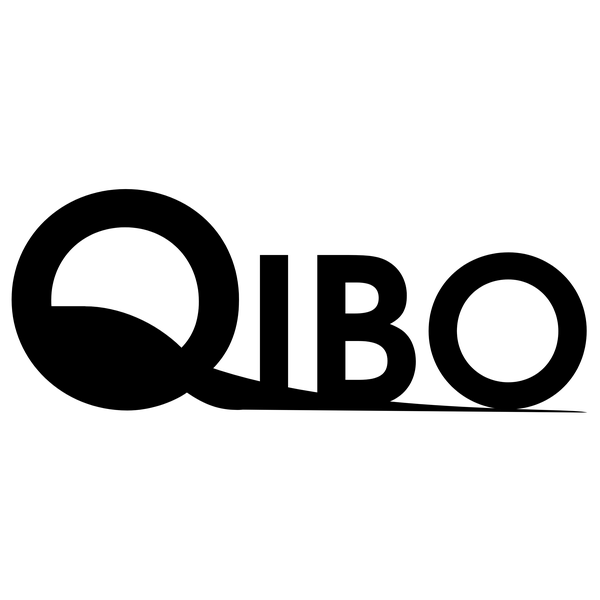
\includegraphics[width=.15\textwidth]{figures/qibo.png} 

\includegraphics[width=.15\textwidth]{figures/unimi.png} 

\includegraphics[width=.15\textwidth]{figures/cern.png}  

\includegraphics[width=.15\textwidth]{figures/qti.png}  

\includegraphics[width=.15\textwidth]{figures/tii.png}  
};
\end{tikzpicture}
}


\begin{document}

\maketitle

\section{Quantum Computing using \texttt{Qibo}}

\begin{frame}[fragile]{The aim of \texttt{Qibo}}
\begin{figure}
    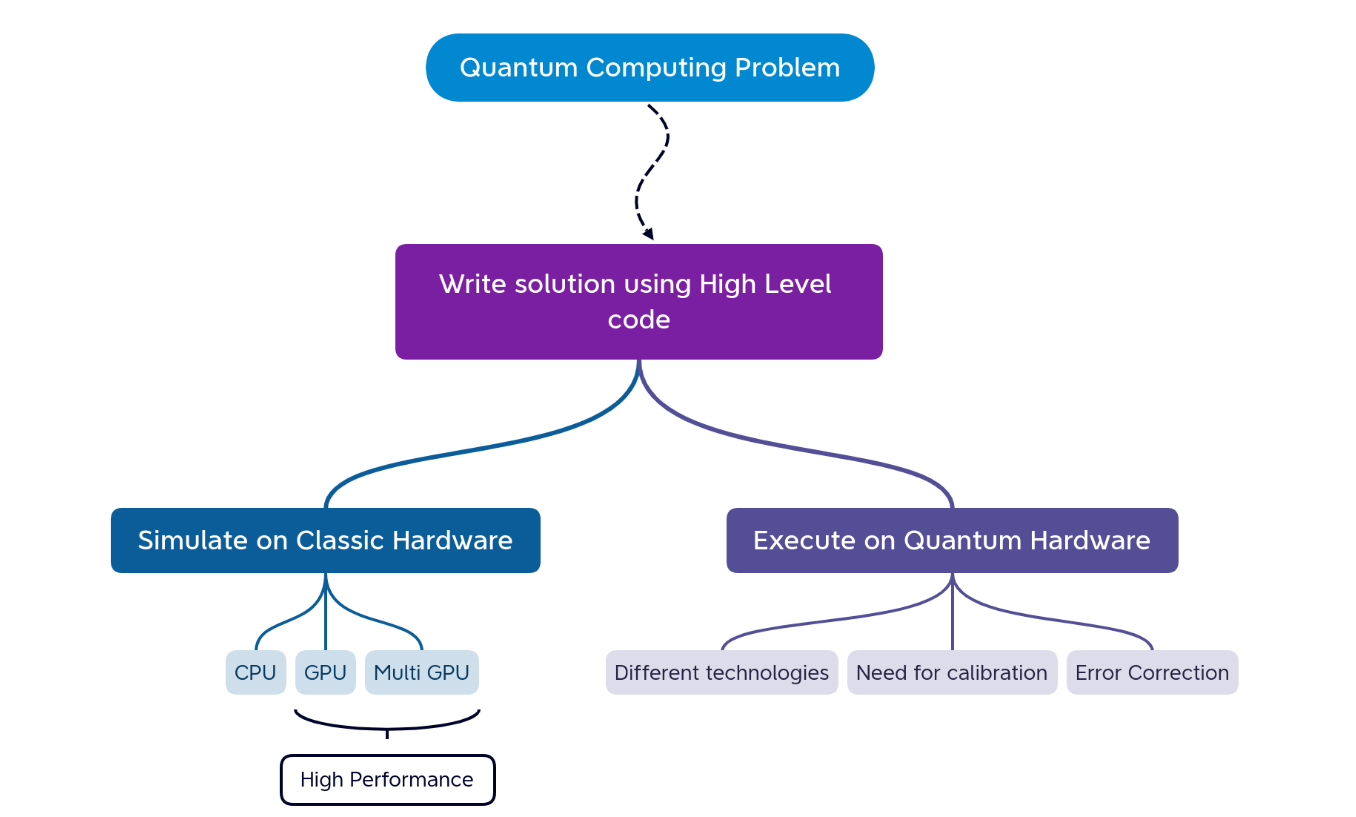
\includegraphics[width=1\textwidth]{figures/qibo_scheme.png}
\end{figure}
\end{frame}

\begin{frame}[fragile]{Contributors at July 2023}
\begin{figure}
    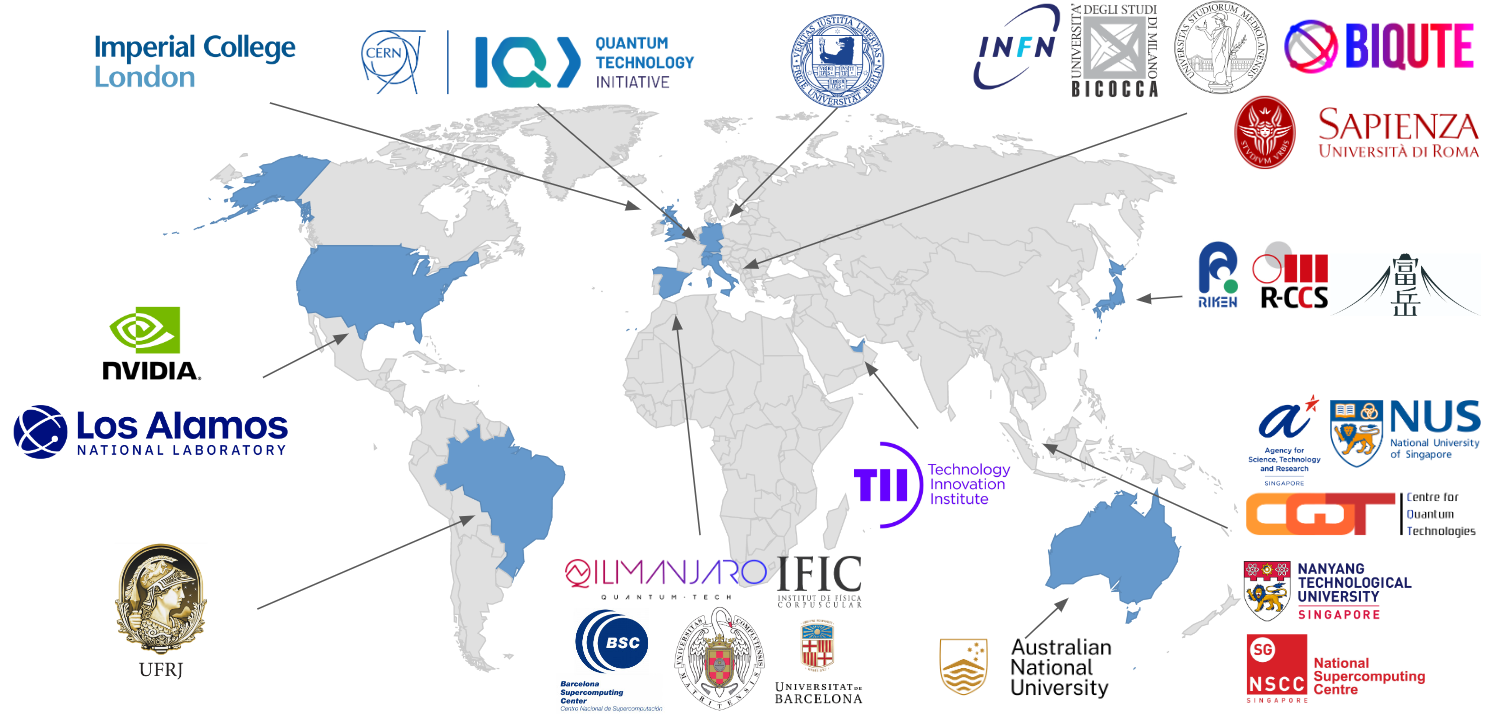
\includegraphics[width=1\textwidth]{figures/qibo_world.png}
\end{figure}
\end{frame}

\begin{frame}[fragile]{High performance quantum simulation}
\begin{figure}
    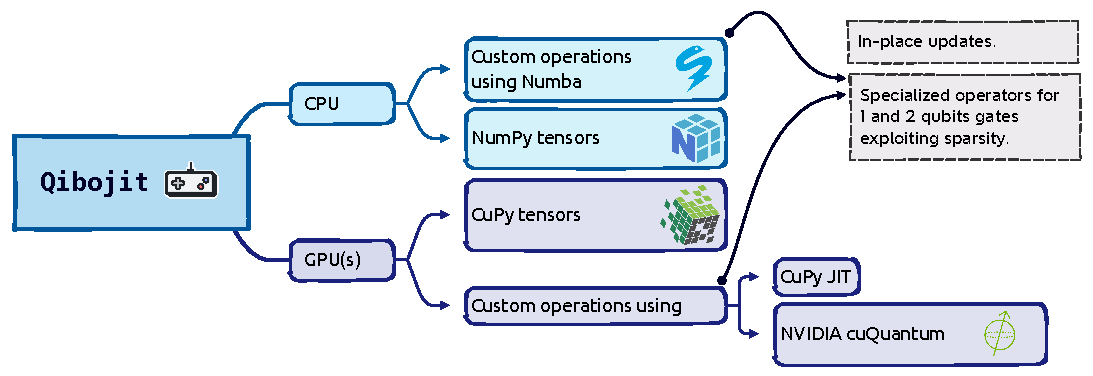
\includegraphics[width=1\textwidth]{figures/qibojit.pdf}
\end{figure}

\faBook\,\, \href{https://arxiv.org/abs/2203.08826}{Quantum simulation with just-in-time compilation, 2022}
\end{frame}


\section{Quantum Machine Learning}

\begin{frame}[fragile]{Variational Quantum Circuits (VQCs)}
\begin{figure}
    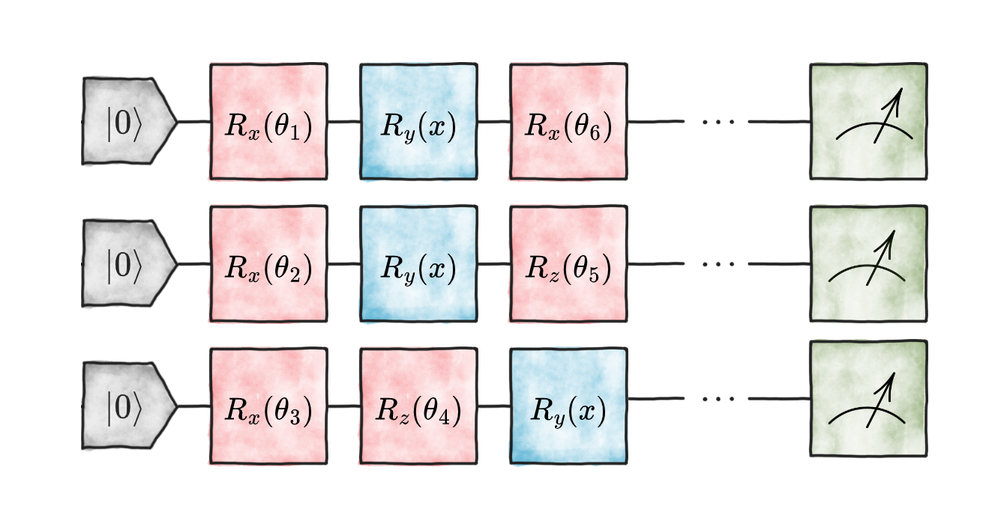
\includegraphics[width=1\textwidth]{figures/vqc.png}
    \caption{\texttt{AKA} a circuit with some parameters, which we call $\mathcal{U}(\bm{\theta}).$}
\end{figure}
\end{frame}

% SLIDE UNO QML
\begin{frame}{Quantum Machine Learning - doing ML using QC}

\vspace{1.5cm}


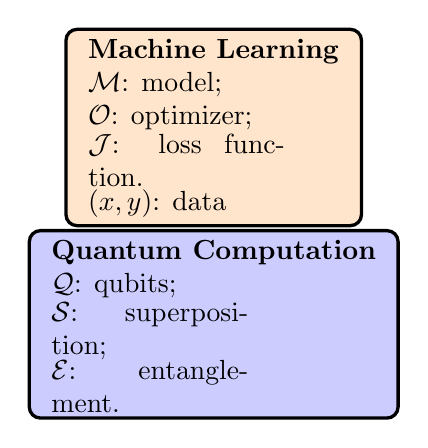
\begin{tikzpicture}[->,>=stealth']

 \node[state, fill=orange!20] (ML) 
 {\begin{tabular}{l}
 \textbf{Machine Learning}\\ 
 \parbox{2.5cm}{$\mathcal{M}$: model;}\\
 \parbox{2.5cm}{$\mathcal{O}$: optimizer;}\\
 \parbox{2.5cm}{$\mathcal{J}$: loss function.}\\
 \parbox{2.5cm}{$(x, y)$: data}
  \end{tabular}
  };
  
  \node[state,
  below of = ML,
  yshift=-1.5cm, fill=blue!20] (QC) 
 {\begin{tabular}{l}
 \textbf{Quantum Computation}\\ 
 \parbox{2.5cm}{$\mathcal{Q}$: qubits;} \\
 \parbox{2.5cm}{$\mathcal{S}$: superposition;}\\
 \parbox{2.5cm}{$\mathcal{E}$: entanglement.}
  \end{tabular}
  };
  
\end{tikzpicture}
\end{frame}


% SLIDE 2 QML
\begin{frame}{Quantum Machine Learning - operating on qubits}

\vspace{1.77cm}

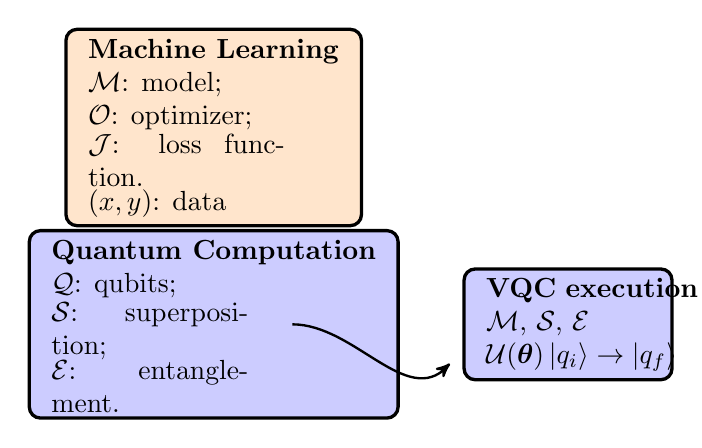
\begin{tikzpicture}[->,>=stealth']

 \node[state, fill=orange!20] (ML) 
 {\begin{tabular}{l}
 \textbf{Machine Learning}\\ 
 \parbox{2.5cm}{$\mathcal{M}$: model;}\\
 \parbox{2.5cm}{$\mathcal{O}$: optimizer;}\\
 \parbox{2.5cm}{$\mathcal{J}$: loss function.}\\
 \parbox{2.5cm}{$(x, y)$: data}
  \end{tabular}
  };
  
  \node[state,
  below of = ML,
  yshift=-1.5cm, fill=blue!20] (QC) 
 {\begin{tabular}{l}
 \textbf{Quantum Computation}\\ 
 \parbox{2.5cm}{$\mathcal{Q}$: qubits;} \\
 \parbox{2.5cm}{$\mathcal{S}$: superposition;}\\
 \parbox{2.5cm}{$\mathcal{E}$: entanglement.}
  \end{tabular}
  };
  
   \node[state,
    right of=QC,
    yshift=0cm,
    anchor=center,
    node distance=4.5cm, 	
    text width=2.5cm, fill=blue!20] (VQC) 
 {%
 \begin{tabular}{l}
  \textbf{VQC execution}\\
  $\mathcal{M}$, $\mathcal{S}$, $\mathcal{E}$ \\
  \parbox{2.8cm}{$\mathcal{U}(\bm{\theta})\ket{q_i} \to \ket{q_f}$}
 \end{tabular}
 };
 
  \draw[line width=0.3mm] (1, -2.5)  to[out=0, in=230] (3, -3);
\end{tikzpicture}

\end{frame}

% SLIDE 3 QML
\begin{frame}{Quantum Machine Learning - natural randomness}

\vspace{1.77cm}

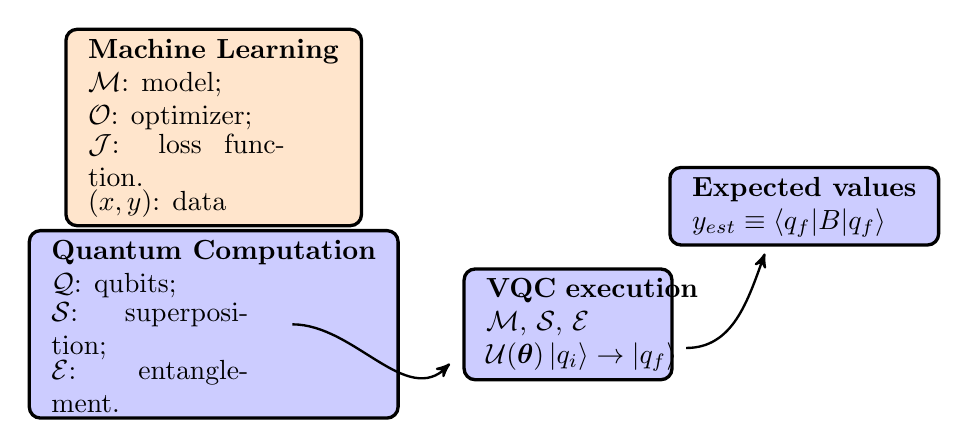
\begin{tikzpicture}[->,>=stealth']

 \node[state, fill=orange!20] (ML) 
 {\begin{tabular}{l}
 \textbf{Machine Learning}\\ 
 \parbox{2.5cm}{$\mathcal{M}$: model;}\\
 \parbox{2.5cm}{$\mathcal{O}$: optimizer;}\\
 \parbox{2.5cm}{$\mathcal{J}$: loss function.}\\
 \parbox{2.5cm}{$(x, y)$: data}
  \end{tabular}
  };
  
  \node[state,
  below of = ML,
  yshift=-1.5cm, fill=blue!20] (QC) 
 {\begin{tabular}{l}
 \textbf{Quantum Computation}\\ 
 \parbox{2.5cm}{$\mathcal{Q}$: qubits;} \\
 \parbox{2.5cm}{$\mathcal{S}$: superposition;}\\
 \parbox{2.5cm}{$\mathcal{E}$: entanglement.}
  \end{tabular}
  };
  
   \node[state,
    right of=QC,
    yshift=0cm,
    anchor=center,
    node distance=4.5cm, 	
    text width=2.5cm, fill=blue!20] (VQC) 
 {%
 \begin{tabular}{l}
  \textbf{VQC execution}\\
  $\mathcal{M}$, $\mathcal{S}$, $\mathcal{E}$ \\
  \parbox{2.8cm}{$\mathcal{U}(\bm{\theta})\ket{q_i} \to \ket{q_f}$}
 \end{tabular}
 };
 
\node[state,
  right of = VQC,
  node distance = 3cm,
  yshift=1.5cm, fill=blue!20] (NSHOT) 
 {\begin{tabular}{l}
 \textbf{Expected values}\\ 
 $y_{est} \equiv \braket{q_f|B|q_f}$
  \end{tabular}
  };
 
\draw[line width=0.3mm] (1, -2.5)  to[out=0, in=230] (3, -3);
\draw[line width=0.3mm] (6, -2.8)  to[out=0, in=250] (7, -1.6);
\end{tikzpicture}

\end{frame}


% SLIDE 4 QML

\begin{frame}{Quantum Machine Learning - encoding the problem}

\vspace{1.01cm}
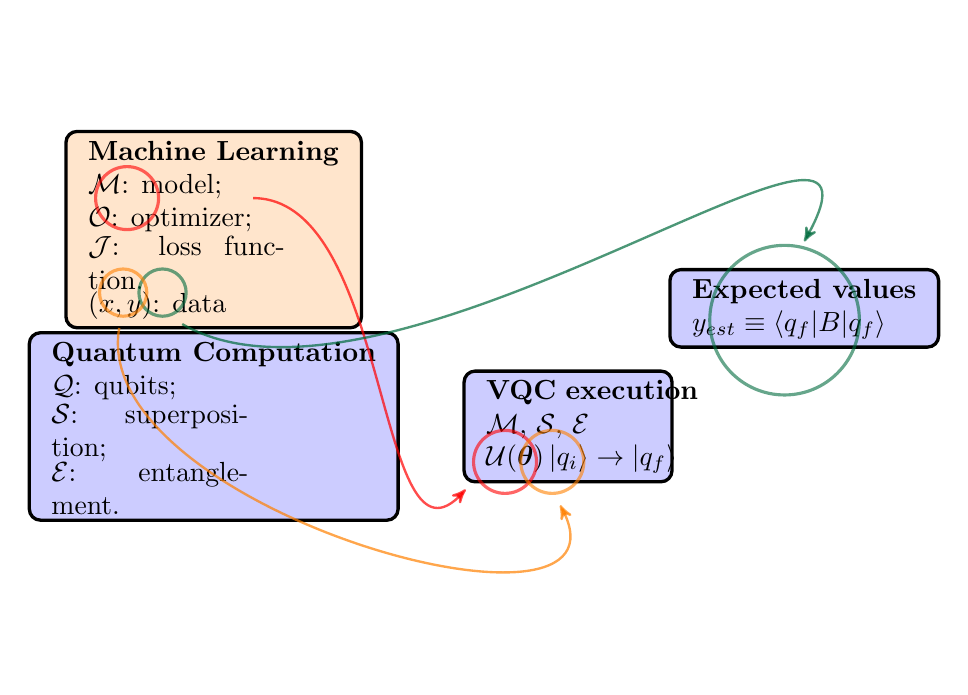
\begin{tikzpicture}[->,>=stealth']

 \node[state, fill=orange!20] (ML) 
 {\begin{tabular}{l}
 \textbf{Machine Learning}\\ 
 \parbox{2.5cm}{$\mathcal{M}$: model;}\\
 \parbox{2.5cm}{$\mathcal{O}$: optimizer;}\\
 \parbox{2.5cm}{$\mathcal{J}$: loss function.}\\
 \parbox{2.5cm}{$(x, y)$: data}
  \end{tabular}
  };
  
  \node[state,
  below of = ML,
  yshift=-1.5cm, fill=blue!20] (QC) 
 {\begin{tabular}{l}
 \textbf{Quantum Computation}\\ 
 \parbox{2.5cm}{$\mathcal{Q}$: qubits;} \\
 \parbox{2.5cm}{$\mathcal{S}$: superposition;}\\
 \parbox{2.5cm}{$\mathcal{E}$: entanglement.}
  \end{tabular}
  };
  
 
 \node[state,
    right of=QC,
    yshift=0cm,
    anchor=center,
    node distance=4.5cm, 	
    text width=2.5cm, fill=blue!20] (VQC) 
 {%
 \begin{tabular}{l}
  \textbf{VQC execution}\\
  $\mathcal{M}$, $\mathcal{S}$, $\mathcal{E}$ \\
  \parbox{2.8cm}{$\mathcal{U}(\bm{\theta})\ket{q_i} \to \ket{q_f}$}
 \end{tabular}
 };
 
\node[state,
  right of = VQC,
  node distance = 3cm,
  yshift=1.5cm, fill=blue!20] (NSHOT) 
 {\begin{tabular}{l}
 \textbf{Expected values}\\ 
 $y_{est} \equiv \braket{q_f|B|q_f}$
  \end{tabular}
  };

  
 \draw[line width=0.3mm, red, opacity = 0.7] (0.5, 0.4)  to[out=0, in=230] (3.2, -3.3);
 \draw[line width=0.3mm, orange, opacity = 0.7] (-1.2, -1.25)  to[out=260, in=300] (4.4, -3.5);
 \draw[line width=0.3mm, cadmiumgreen, opacity = 0.7] (-0.4, -1.2)  to[out=330, in=60] (7.5, -0.15);
  
 
 \draw[red, line width=0.4mm, opacity = 0.6] (3.7,-2.95) circle (0.4 cm);
 \draw[red, line width=0.4mm, opacity = 0.6] (-1.1, 0.4) circle (0.4 cm);
 \draw[cadmiumgreen, line width=0.4mm, opacity = 0.6] (-0.65,-0.8) circle (0.3 cm);
 \draw[cadmiumgreen, line width=0.4mm, opacity = 0.6] (7.25,-1.15) circle (0.95 cm);
 \draw[orange, line width=0.4mm, opacity = 0.6] (4.3,-2.95) circle (0.4 cm);
 \draw[orange, line width=0.4mm, opacity = 0.6] (-1.15,-0.8) circle (0.3 cm);


\end{tikzpicture}
\end{frame}

% SLIDE 5 QML

\begin{frame}{Quantum Machine Learning!}

\vspace{0.25cm}
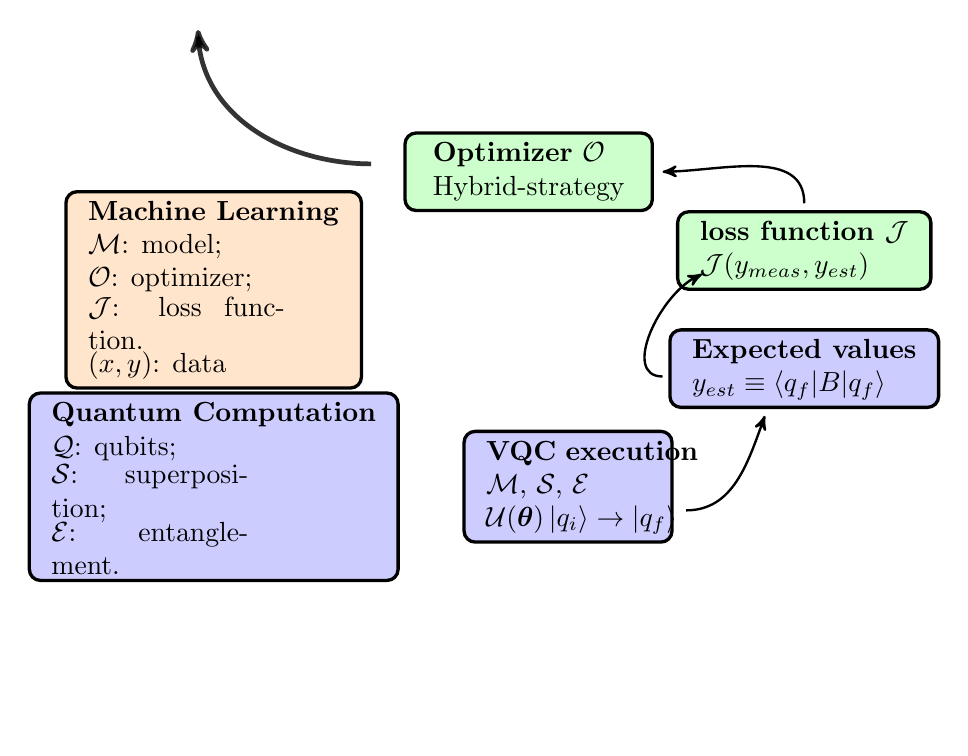
\begin{tikzpicture}[->,>=stealth']


 \node[state, fill=orange!20] (ML) 
 {\begin{tabular}{l}
 \textbf{Machine Learning}\\ 
 \parbox{2.5cm}{$\mathcal{M}$: model;}\\
 \parbox{2.5cm}{$\mathcal{O}$: optimizer;}\\
 \parbox{2.5cm}{$\mathcal{J}$: loss function.}\\
 \parbox{2.5cm}{$(x, y)$: data}
  \end{tabular}
  };
  
  \node[state,
  below of = ML,
  yshift=-1.5cm, fill=blue!20] (QC) 
 {\begin{tabular}{l}
 \textbf{Quantum Computation}\\ 
 \parbox{2.5cm}{$\mathcal{Q}$: qubits;} \\
 \parbox{2.5cm}{$\mathcal{S}$: superposition;}\\
 \parbox{2.5cm}{$\mathcal{E}$: entanglement.}
  \end{tabular}
  };
  

 \node[state,   
  text width=3cm, 
  yshift=1.5cm, 
  right of=ML, 	
  node distance=4cm, 
  anchor=center, fill=green!20] (OPT) 
 {%
 \begin{tabular}{l} 	% content
  \textbf{Optimizer $\mathcal{O}$}\\
  Hybrid-strategy
 \end{tabular}
 };
 
 \node[state,
    right of=QC,
    yshift=0cm,
    anchor=center,
    node distance=4.5cm, 	
    text width=2.5cm, fill=blue!20] (VQC) 
 {%
 \begin{tabular}{l}
  \textbf{VQC execution}\\
  $\mathcal{M}$, $\mathcal{S}$, $\mathcal{E}$ \\
  \parbox{2.8cm}{$\mathcal{U}(\bm{\theta})\ket{q_i} \to \ket{q_f}$}
 \end{tabular}
 };
 
\node[state,
  right of = VQC,
  node distance = 3cm,
  yshift=1.5cm, fill=blue!20] (NSHOT) 
 {\begin{tabular}{l}
 \textbf{Expected values}\\ 
 $y_{est} \equiv \braket{q_f|B|q_f}$
  \end{tabular}
  };
  
  \node[state,
  above of = NSHOT,
  node distance = 1.5cm,
  yshift=0cm, fill=green!20] (J) 
 {\begin{tabular}{l}
 \textbf{loss function $\mathcal{J}$}\\ 
 $\mathcal{J}(y_{meas}, y_{est})$
  \end{tabular}
  };
  

 \draw[line width=0.3mm] (6, -2.8)  to[out=0, in=250] (7, -1.6);
 \draw[line width=0.3mm] (5.7, -1.1)  to[out=180, in=200] (6.2, 0.2);
 \draw[line width=0.3mm] (7.5, 1.1)  to[out=90, in=0] (5.7, 1.5);
 \draw[line width=0.6mm, opacity=0.8] (2, 1.6)  to[out=180, in=270] (-0.2, 3.3);
 
 \draw[line width=0.3mm, orange, opacity = 0.0] (-1.2, -1.25)  to[out=260, in=300] (4.4, -3.5);

\end{tikzpicture}

\end{frame}

\begin{frame}{Why QML?}
\large
  \begin{itemize}
  \item<2,3,4,5>[\faMoney] \textbf{shallow models} thanks to superposition and entanglement;
  \item<3,4,5>[\faCubes] map problems into Hilbert's spaces loads to high \textbf{expressivity};
  \item<4,5>[\faTachometer] exploit QC sub-routines to \textbf{speed-up} classical algorithms (e.g. using
  Grover);
  \item<5>[\faRocket] physical advantages when dealing with \textbf{combinatorial optimization} (quantum annealing).
  \end{itemize}
  \begin{multicols}{4}
    \begin{figure}
       \uncover<2,3,4,5>{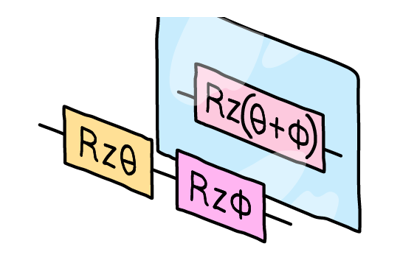
\includegraphics[height=2cm, width=0.25\textwidth]{figures/shallow.png}}%
    \end{figure}
    \begin{figure}
       \uncover<3,4,5>{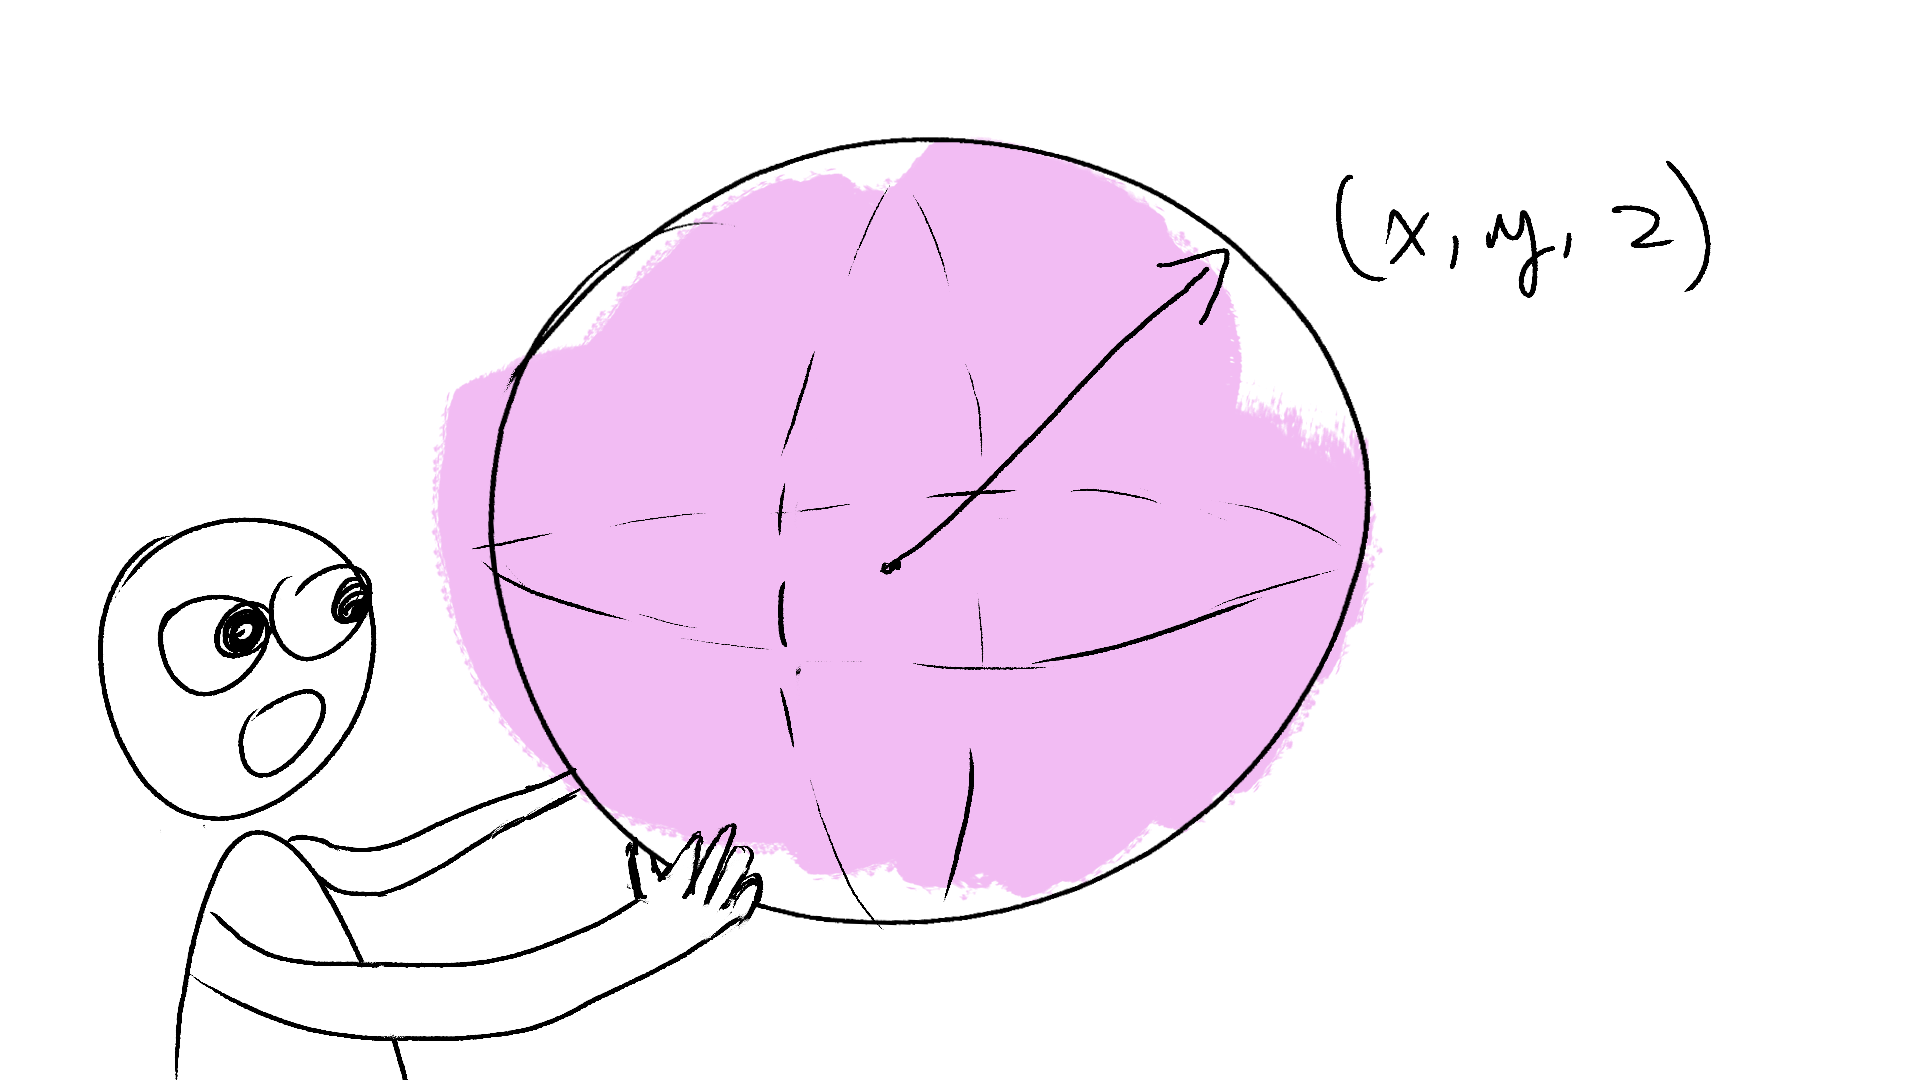
\includegraphics[height=2cm, width=0.25\textwidth]{figures/block_sphere.png}}%
    \end{figure}
    \begin{figure}
       \uncover<4,5>{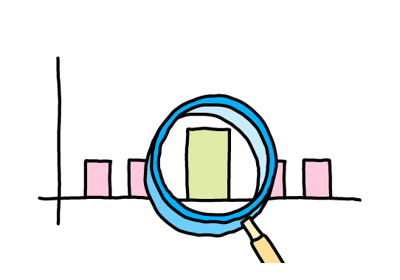
\includegraphics[height=2cm, width=0.25\textwidth]{figures/speedup.png}}%
    \end{figure}
    \begin{figure}
       \uncover<5>{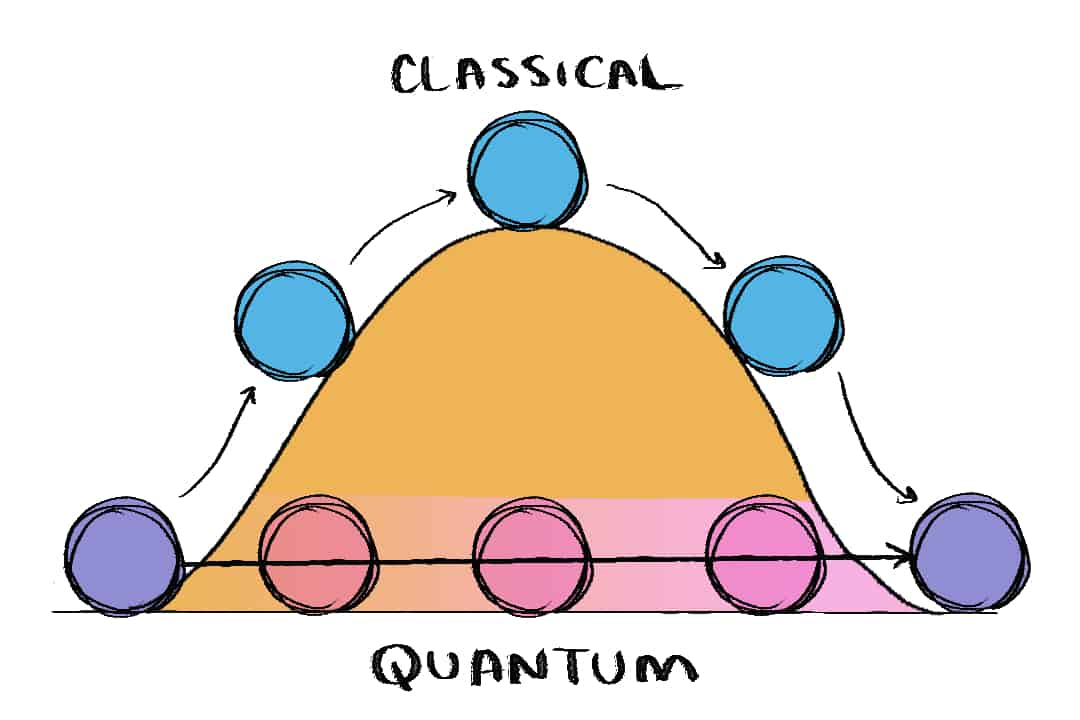
\includegraphics[height=2cm, width=0.25\textwidth]{figures/tunneling.jpg}}%
    \end{figure}
    \end{multicols}
\end{frame}

\begin{frame}{Rational}
Using Variational Quantum Circuits we define a Variational Quantum Computer!
\pause
\begin{multicols}{2}
\begin{itemize}
\item<2,3,4>[1.] we want a quantum circuit $\mathcal{U}(\bm{\theta})$ to approximates some law $V$;
\item<3,4>[2.] executing $\mathcal{U}(\bm{\theta})$ we use a variational quantum state
to reach the solution;
\item<4>[3.] \textbf{Solovay-Kitaev theorem}: the number of gates needed by $\mathcal{U}$ to 
represent $V$ with precision $\delta$ is $\mathcal{O}(\log^c \delta^{-1})$, where
$c<4$.
\end{itemize}
\begin{figure}
    \uncover<2,3,4>{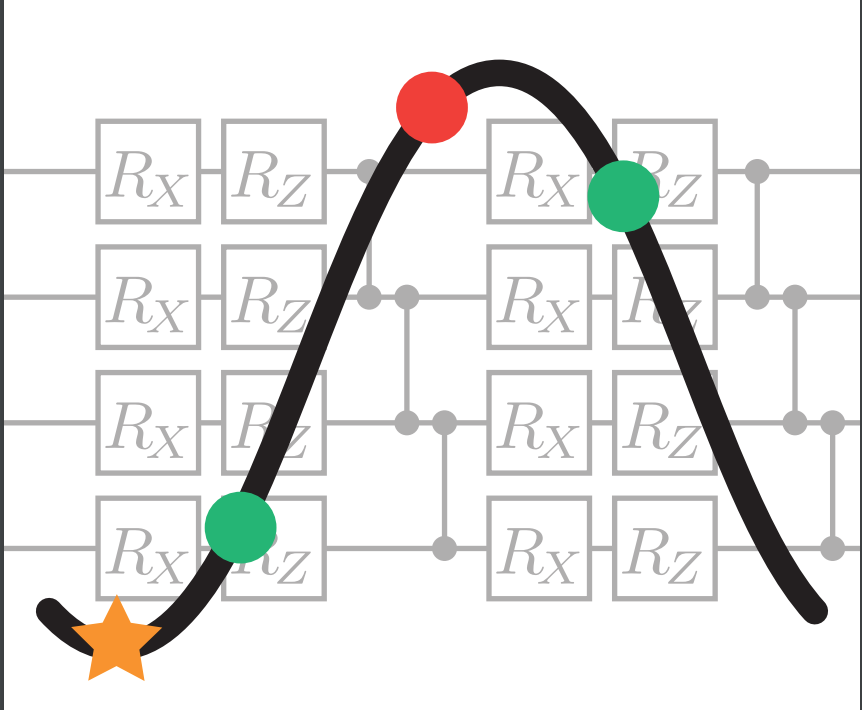
\includegraphics[width=0.5\textwidth]{figures/variational.png}}
\end{figure}
\end{multicols}

\end{frame}

\end{document}
